\documentclass[conference]{IEEEtran}

% Package imports
\usepackage{graphicx}
\usepackage{amsmath}
\usepackage{hyperref}

% Title and author
\title{Security Measures in Cellular Networks: How Good Are They}

% Document begins
\begin{document}
\maketitle

% Abstract
\begin{abstract}
 Numerous applications, including online banking, mobile payments, and real-time information sharing, are made possible by cellular networks, which are becoming an essential component of contemporary communication systems. But the increased dependence on these networks has made them vulnerable to serious security threats. The security features and weaknesses of the three main cellular network generations—GSM, LTE, and 5G—are surveyed in this study. We analyze the architecture of these networks, and investigate the attacks which are possible against these networks such as eavesdropping, rogue base stations, and cryptographic breaches and survey the security mechanism of these networks. Finally, we have reviewed the security mechanism of all the networks.

\end{abstract}

% Introduction
\section{Introduction}
The growth of cellular networks, from GSM to LTE and now 5G, has transformed worldwide communication by providing quicker and more dependable access. However, this advancement has created severe security challenges. Protecting user privacy, preserving data integrity, and ensuring service availability are vital since these networks power critical systems such as healthcare and finance.
GSM established the groundwork for basic encryption, LTE enhanced security with mutual authentication and stronger protocols, and 5G brought sophisticated safeguards to solve earlier flaws and counter emerging threats from increasing connectivity and IoT integration. Despite these developments, cellular networks remain vulnerable to assaults such as eavesdropping, impersonation, and denial-of-service.
This article discusses GSM, LTE, and 5G networks, examines their security measures, assesses their effectiveness in reducing attacks, and analyses their weaknesses. It examines the strengths and shortcomings of each generation, using real-world examples, and analyses how future networks can improve security.
 

% AMAN ----SECTION
\section{GSM}
\subsection{Overview of GSM Network Architecture}
The architecture of a GSM network is divided into several functional components, each designed for specific purposes. Figure 1 illustrates the key components of the GSM network, which can be broadly categorized into three main sections: the Mobile Station (MS), the Base Station Subsystem (BSS), and the Switching System (SS). \cite{kaur2012review}

\begin{figure}
    \centering
    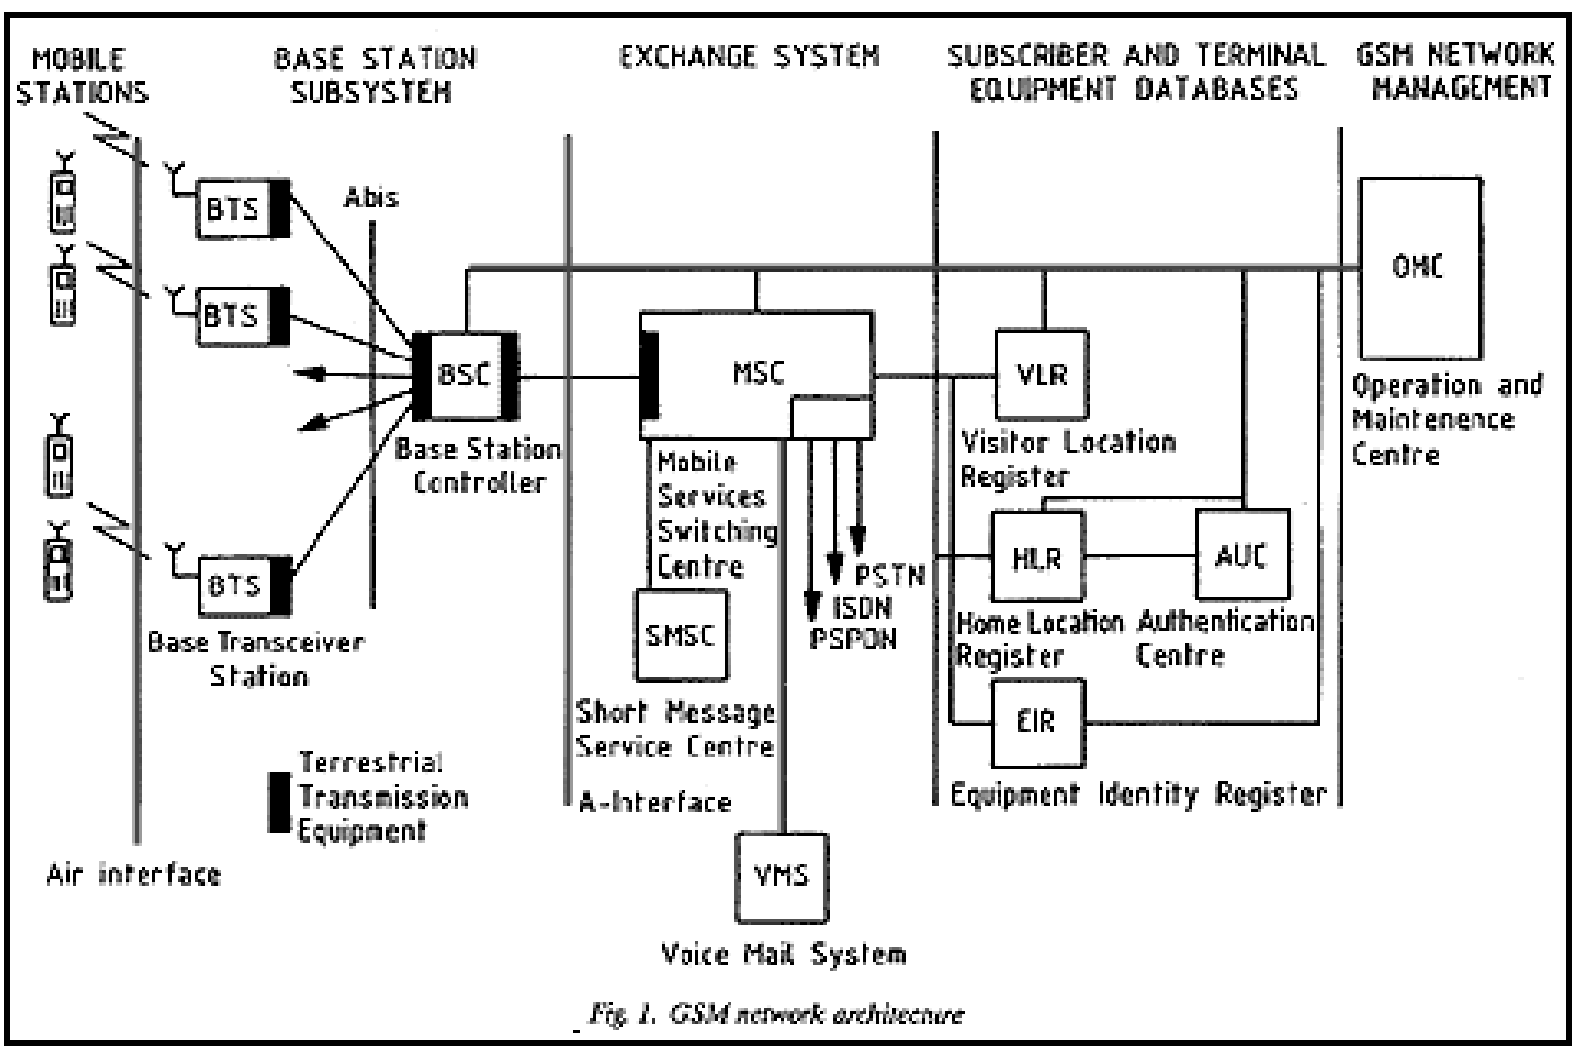
\includegraphics[width=0.5\linewidth]{Assets/GSM-Architecture.png}
    \caption{GSM Architecture} \cite{kaur2012review}
    \label{fig:enter-label}
\end{figure}

\begin{itemize}
    \item \textbf{Mobile Station (MS)} : The Mobile Station consists of two essential parts:
    \begin{itemize}
        \item \textbf{Mobile Equipment (ME)}: A portable, handheld, or vehicle-mounted device uniquely identified by its IMEI (International Mobile Equipment Identity). This device facilitates both voice and data communication.
        \item \textbf{Subscriber Identity Module (SIM)}: A smart card that contains the IMSI (International Mobile Subscriber Identity). It enables users to make and receive calls and access subscribed services. The SIM card is secured by a PIN and can be transferred between devices, carrying the necessary information to activate the phone.
        \item \textbf{Base Station Subsystem (BSS)}: A smart card that contains the IMSI (International Mobile Subscriber Identity). It enables users to make and receive calls and access subscribed services. The SIM card is secured by a PIN and can be transferred between devices, carrying the necessary information to activate the phone.
    \end{itemize}

    \item \textbf{Base Station Subsystem (BSS)} : The BSS is responsible for managing radio-related functions and comprises the following components:
    \begin{itemize}
        \item \textbf{Base Station Controller (BSC)} : This component manages control functions and physical connections between the MSC and BTS. It acts as a high-capacity switch, handling tasks like handovers, cell configuration data, and regulating RF power levels in the BTS. A single MSC can serve multiple BSCs.

        \item \textbf{Base Transceiver Station (BTS)}: This equipment establishes the radio interface with the mobile station. It includes the necessary transceivers and antennas to serve individual cells in the network. A BSC controls a group of BTSs.        
    \end{itemize}

    \item \textbf{Switching System (SS)} : The Switching System handles call processing and subscriber management tasks. It includes the following units:
    \begin{itemize}
        \item \textbf{Home Location Register (HLR)}: A critical database for storing and managing subscription data. It maintains permanent subscriber information, including service profiles, location data, and activity status. When a user subscribes to a network operator, their details are recorded in the operator's HLR.

        \item \textbf{Mobile Services Switching Center (MSC)}: The MSC is the core telephony switch, managing call routing between different telephone and data systems. It also oversees functions like toll ticketing, network interfacing, and common channel signaling.

        \item \textbf{Visitor Location Register (VLR)}: A temporary database integrated with the MSC that stores information about roaming subscribers. When a mobile device enters a new MSC area, the VLR requests details from the HLR. This ensures call setup can occur without repeatedly querying the HLR.

        \item \textbf{Authentication Center (AUC)}: The AUC generates authentication and encryption parameters to verify subscriber identity and maintain call confidentiality. It also safeguards operators against fraud.

        \item \textbf{Equipment Identity Register (EIR)}: The EIR is a database containing details about mobile equipment to prevent unauthorized, stolen, or faulty devices from accessing the network. The AUC and EIR can be implemented as standalone units or combined into a single node.

    \end{itemize}
    
\end{itemize}

\subsection{Security Measures in GSM}
\begin{itemize}
    \item \textbf{Authentication}: 
    
    \begin{itemize}
        
        \item \textbf{Generating authentication vectors}:
        Before understanding how the authentication works in GSM, we need to understand how the authentication vectors or security parameters are generated.
        The two key elements in our network dealing with authentication are 
        \begin{itemize}
            \item \text{SIM - Subscriber Identity Module}
            \item \text{AuC - Authentication Center}
        \end{itemize}
        Inside both elements we use 2 mathematical algorithms called A3 and A8. These algorithms are secret and are specific to given service providers. There is also a 128 bit subscriber authentication key which is present in both of them which is called Ki. 
    
        In AuC, a random number termed RAND is generated, which is fed to A3 and A8 algorithms to generate SRES (Signal Response) and Kc (cipher key)  respectively. (Please refer to the image below).
        Thus, SRES, Kc and RAND together are termed as authentication vector. \cite{kaur2012review}

        \begin{figure}
            \centering
            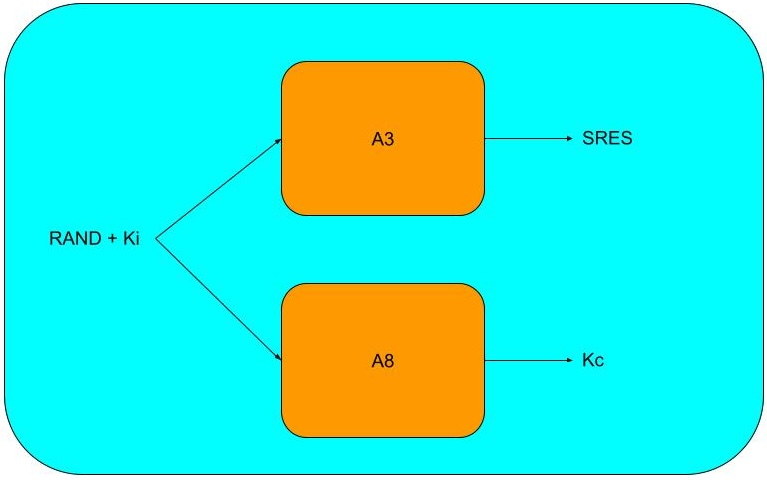
\includegraphics[width=0.5\linewidth]{Assets/GSM-Auth-1.jpg}
            \caption{Generation of SRES and Kc}
            \label{fig:enter-label}
        \end{figure}

        \item \textbf{Working of Authentication in GSM}:
        \begin{enumerate}
            \item Initiating the Authentication Process:
            When a mobile device (user) attempts to connect to the network, it sends its IMSI (International Mobile Subscriber Identity).

            \item Processing at AuC:
            Upon receiving the IMSI, the network checks its database to retrieve the subscriber's secret key (Ki) from the Authentication Center (AuC) and calculate the Random number (RAND), Signal response (SRES) and Cipher Key (Kc).

            \item Processing at SIM:
            The MSC sends the authentication request to the Mobile station and this request message contains RAND. This RAND is used by SIM along with Ki to generate the SRES and KC using A3 and A8 algorithms. These values which are generated by the SIM card are sent back to MSC as a response.

            \item Verification at MSC:
            MSC then compares SRES generated by the SIM with the SRES which it got from AuC. If they are the same then the subscriber is authenticated.

            \item Establishing secure connection:
            The derived ciphering key Kc is used for encrypting communication between the mobile device and the network. 
        \end{enumerate}
        
    \end{itemize}

    \item \textbf{Encryption}: 
    Once the subscriber is authenticated, the cipher key Kc which is generated by SIM using RAND (Number generated by AuC) and Ki ( subscriber authentication key ) when fed to A8 Algorithm, is now used for encrypting the communication between mobile device and the network.
    Encrypted voice and data communication between the mobile station (MS) and the network is achieved using the A5 ciphering algorithm. 
    The MSC will additionally store the encryption key in the base station (via the BSC) for use in encryption and decryption processes if the authentication result is accepted. The mobile system is then given an encryption mode command, or "test signal," by the BSC. 
    The mobile system should respond by sending out an encrypted signal (encryption mode complete), which, if deciphered by the BSC, allows for ongoing communication and signalling. \cite{margrave1999gsm}

\subsection{Attacks in GSM}
\begin{itemize}
    \item SIM Attacks: The GSM SIM is intended to be copy proof and tamper proof. But over the period of time, as more and more vulnerabilities
    of SIM are getting discovered, it no longer remain secure. The SIM cloning is possible and the attacker needs certain 
    hardware and physical access to the target SIM. In particular, the attacker must have a SIM reader, a SIM software program, and a SIM chip writer \cite{quirke2004security} \cite{sidharsancomplete}.
    Physical SIM cloning is limited to the common and basic encryption algorithm called COMP128V1 \cite{quirke2004security} \cite{sidharsancomplete}. The COMP128v1 algorithm has weaknesses which allow an attacker 
    to successfully mount a brute force attack and then extract the secret individual subscriber authentication key (Ki) of the SIM, along with the International Mobile Subscriber Identity (IMSI) and Integrated Circuit Card Identifier (ICCID).
    \cite{singh2013gsm}

    \item Encryption : The A5/1 or A5/2 encryption algorithms are used to encrypt data in the GSM network. A5/0 is used in nations with political barriers to the provision of cryptographic hardware and does not employ encryption.
    The former Soviet Union and a few Middle Eastern nations are two examples of this. 
    Mathematicians and cryptography experts have examined A5/1, which is supposedly the more robust of the two algorithms in use, and found it to be extremely vulnerable to cryptanalytic attacks.
    Several researchers such as M. Briceno, R. Anderson, M. Roe and J. Golic 9 also explored different aspects of the algorithm as well as different types of attacks on it. 
    And these attacks have become the most widespread among those that are directed at the algorithm. Some examples of these attacks are the Baised Birthday Attack and the Random Sub graph Attack. 
    The first attack requires two minutes of data and one minute of processing while the second attack two seconds of data and several minutes of processing. \cite{lord2003modern}
    
    The COMP 128 algorithm used for A3/A8 has many vulnerabilities and this makes it possible to obtain the Ki and the IMSI and
    these can be successfully used to program another \cite{rao2002partitioning}

    \item SMS Spoofing : SMS spoofing is a significant and realistic threat as it allows attackers to inject fraudulent SMS messages into the network using fake originator IDs.
    By sending an SMS from the internet with the correct headers, an attacker can impersonate a legitimate Mobile Equipment (ME). Since the ME cannot differentiate between a genuine message and one originating from the internet, it processes the message as legitimate, enabling the attacker to manipulate transactions as desired.

    \item Denial-of-Service (DoS) Attack : In mobile networks, flooding a device with SMS messages can render it ineffective by overloading the signaling layer, which handles essential network tasks. 
    A specific form of this, the "Silent" SMS DoS attack, goes unnoticed by the victim. Its symptoms include rapid battery drain and an inability to receive calls, as the signaling channel becomes clogged. 
    This type of attack may be used for economic gain, to prevent communication between parties, or to ensure critical notifications are missed.
 
\end{itemize}
    
\end{itemize}

% AMAN - END


% SOURAV ---- SECTION
\section{LTE}
\subsection{Overview of LTE Network Architecture}
The architecture of a LTE network is divided into different functional components, each component is designed for specific purposes. Figure \ref{fig:lte_architecture} demonstrates the major components of the LTE network, which is composed of 3 major components: the User Equipment (UE), the Evolved Universal Terrestrial Radio Access Network (E-UTRAN), and the Evolved Packet Core (EPC).

    

\begin{itemize}
    \item \textbf{User Equipment (UE)} : The Mobile Station consists of two essential parts:
    \begin{itemize}
        \item \textbf{Mobile Operating System }: The general-purpose system users interact with (e.g. Android, IOS).
        \item \textbf{Telephony Subsystem}: It includes a baseband processor, which has its own operating system developed by the cellular SoC manufacturer to handle network communication\cite{cichonski2016guide}.

    
    \item  \textbf{Key components and identifiers in UE} : The Universal Integrated Circuit Card (UICC), a smart card inserted into the Mobile Equipment (ME) that stores personal data, cryptographic keys, and runs Java applications for network access; the International Mobile Equipment Identifier (IMEI), which uniquely identifies the device to the network; and the International Mobile Subscriber Identity (IMSI), which identifies the subscriber\cite{cichonski2016guide}.


    
\end{itemize}
    \item \textbf{E-UTRAN} : UEs connect to the E-UTRAN to send data to the core network. The E-UTRAN is a mesh network composed of base stations. A base station, or Evolved Node B (eNodeB), modulates and demodulates radio signals to communicate with UEs. eNodeBs serves as a relay point to transmit IP packets to and from the man network. eNodeBs use the X2 interface to communicate with each other\cite{cichonski2016guide}. E-UTRAN comprises the following components: 

    
        
    \begin{itemize}
        \item \textbf{Evolved Node B (eNodeB or eNB)} : A base station is an eNodeB.
     
    \end{itemize}

    \item \textbf{Evolved Packet Core (EPC)} : It is the most important component in LTE. It handles calls processing and subscriber management tasks. Following units are included in EPC:
    \begin{itemize}
        \item \textbf{Mobility Management Entity (MME)} : It is the main signaling node and does not engage with user traffic. It handles a wide range of capabilities, such as choosing the S-GW and P-GWs, sending pages, managing/storing UE contexts, generating temporary IDs, and controlling authentication procedures\cite{cichonski2016guide}.

        \item \textbf{Serving Gateway (S-GW)} : Routes data between the P-GW and the E-UTRAN, anchors UEs for intra-eNodeB handoffs, and carries user plane data\cite{cichonski2016guide}.

        \item \textbf{Packet Data Network Gateway (P-GW) } : It connects to non-3GPP networks, routes packets, and assigns IP addresses\cite{cichonski2016guide}.

        \item \textbf{Home Subscriber Server (HSS) } : Holds the secret key K and is a master database containing subscriber data\cite{cichonski2016guide}.

        \item \textbf{Authentication Center (AuC) } : It is located inside the HSS, it executes cryptographic computations during authentication and associates long-term identities with pre-shared cryptographic keys\cite{cichonski2016guide}.

        \item \textbf{Policy and Charging Rules Function (PCRF) } : The PCRF distributes and enforces rules and regulations to the P-GW concerning billing, network resource access, and quality of service (QoS)\cite{cichonski2016guide}.

\begin{figure}
            \centering
            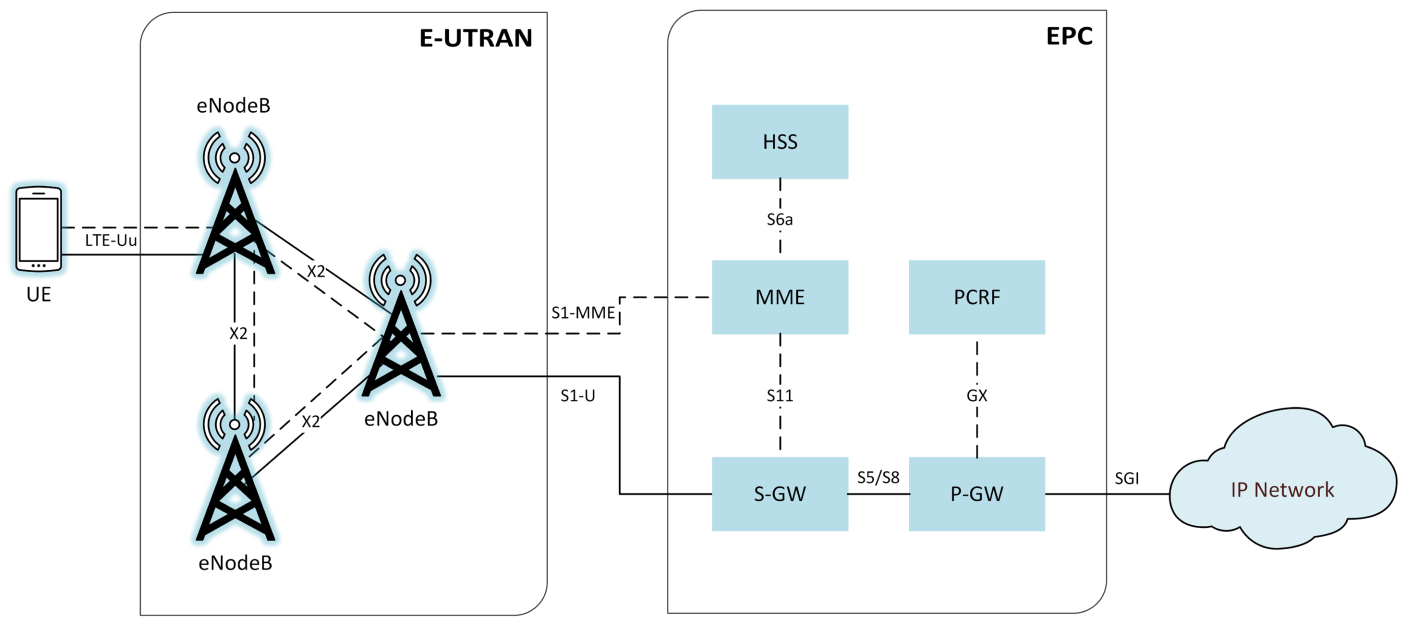
\includegraphics[width=0.9\linewidth]{Assets/lte_architecture.png}
            \caption{Architecture of LTE Network} \cite{cichonski2016guide}
            \label{fig:lte_architecture}
        \end{figure}
    \end{itemize}
    
\end{itemize}

\subsection{Security Measures in LTE}
The LTE security framework is designed to provide robust protection for user data and signaling while addressing the unique requirements of modern cellular networks.
\begin{itemize}
    \item \textbf{Cryptography}: 
    Cryptographic algorithms used for confidentiality and authentication in 2G systems, such as A3, A5, and A8, were proprietary. New cryptographic standards EEA1/EIA1 (SNOW 3G), EEA2/EIA2 (AES), and EEA3/EIA3 (ZUC) were added by LTE\cite{cichonski2016guide}. A more intricate key structure that supports 256-bit keys—although many implementations still utilise 128 bits—was also included. Additionally, LTE enhances security and flexibility by enabling distinct cryptographic methods for the control and user planes\cite{cao2013survey}

    \item \textbf{Hardware Security}: 
    The Universal Integrated Circuit Card (UICC) serves as the foundation of LTE's security architecture. The UICC (Universal Integrated Circuit Card) is an advanced SIM card integral to LTE security, hosting the Universal Subscriber Identity Module (USIM) application responsible for critical functions like authentication and cryptographic operations. Equipped with a processor, memory, and network awareness, and can facilitate NFC. The main function of the UICC is storing the pre-shared cryptographic key (K), crucial for LTE's security framework. It is used to derive the session master key (KASME). The UICC collaborates with the HSS and MME for cryptographic operations, subscriber authentication, and storing security contexts. It also secures critical identities like IMSI and IMEI. Additionally, a PIN can be configured on the UICC, preventing unauthorized access if the card is stolen or moved to another device\cite{cichonski2016guide}.

    \item \textbf{UE Authentication in LTE}: 
    LTE uses the Authentication and Key Agreement (AKA) protocol \cite{cao2013survey} to verify that the UICC and the network share the secret key (K)[]. This process ensures mutual authentication between the UICC and the LTE network but does not authenticate the user or device directly. During the attach process, the UE sends its identifier (e.g., IMSI, TMSI, or GUTI) to the MME, which forwards it to the HSS/AuC. The HSS generates an authentication vector (AUTN) using inputs like K, a random nonce (RAND), and a sequence number (SQN)\cite{cichonski2016guide}. This vector, including the expected result (XRES) and AUTN, is sent back to the UE via the MME. The USIM performs cryptographic calculations using K and SQN to produce a response (RES), which is sent to the MME. If RES matches XRES, authentication is successful, granting the UE network access\cite{cao2013survey}.

    \item \textbf{Air Interface Security in LTE}: 
    In LTE, the communication between the User Equipment (UE) and the eNodeB takes place over the air interface (Uu interface), which involves radio frequency (RF) signals. These RF signals can be intercepted, making security critical. The security parameters for a connection are negotiated using the Security Mode Command (SMC). The cryptographic algorithm negotiation between the UE and the network is done, ensuring the selection of appropriate security measures for ciphering, user plane protection, and Non-Access Stratum (NAS) integrity. Security configurations are done separately at the Access Stratum (AS) and NAS levels. Once the security procedures are completed, a security context is established, which stores session keys but not long-term identifiers like IMSI or IMEI. This context can be reused for future connections, reducing unnecessary authentication processes, and minimizing network congestion\cite{cichonski2016guide}.

    \item \textbf{E-UTRAN Security in LTE}: 
    The E-UTRAN connects the UE to the core network in LTE, facilitating essential functions like mobility. A critical feature of E-UTRAN is handover, allowing users to maintain continuous service while moving across different areas. The handover process involves communication between base stations via the X2 interface.There are two types of handovers in LTE: X2 handover and S1 handover. In S1 handover, the MME is aware of the handover in advance, allowing it to refresh cryptographic parameters before the connection is severed. In contrast, X2 handover occurs directly between eNodeBs, with the MME unaware, and fresh keying material is provided only after the handover. During the handover, new session keys are generated to ensure security, but a new master session key (KASME) is not created. The KeNB key is used to generate a new key, KeNB*, which protects the new session post-handover. Importantly, the previous session's keys are not shared between the source eNodeB and the new eNodeB, ensuring the security of the new session\cite{cichonski2016guide}.


    \item \textbf{Backhaul Security}: 
    Backhaul security in LTE networks focuses on safeguarding data transmission between eNodeBs and the Evolved Packet Core (EPC) over the S1 interface. Ensuring physical protection is challenging, as Mobile Network Operators (MNOs) often rely on third-party infrastructure for backhaul connections. Security measures, such as IPsec tunnels with pre-shared keys or digital certificates, help encrypt data over untrusted interfaces\cite{cichonski2016guide}.


\end{itemize}

\subsection{Threats to LTE Network}
The use of LTE network has increased tremendously and so have been the attacks and threats to the LTE network as well. Attacks like Denial of Service(DoS) and Distributed Denial of Service (DDoS) \cite{kamel2014survey}have an affect on availability of the LTE network. Some of the threats are discussed below.

\begin{enumerate}
            \item \textbf{Radio jamming}:
            In order to interfere with communications by lowering the signal to noise ratio, radio jamming is used to hamper the transmission of radio signals.  Finding and stopping the jamming device is one method of stopping this attack\cite{jover2013security}.

            \item \textbf{Jamming Attacks}:
            Jamming attacks disrupt LTE network services by transmitting noise or static over specific frequencies, thus interfering with the communication between User Equipment (UE) and eNodeBs\cite{jover2013security}. Uplink smart jamming us used as it rejects services to all the users which are present in the focused area\cite{jover2014enhancing}.

            \item \textbf{Cryptographic Key Attacks (Attacks Against K)}:
            The cryptographic keys (denoted as 'K') in LTE systems are crucial for ensuring security at multiple levels. If an attacker gains access to this key, they could impersonate subscribers, decrypt communications, and bypass security measures across the network. This could lead to severe privacy breaches and unauthorized access to services\cite{cichonski2016guide}. 

            \item \textbf{Backhaul and Core Eavesdropping}:
            The backhaul connection links the LTE core network to the eNodeBs. If encryption is not used on this critical interface, attackers could intercept and listen to communications between cell sites and the core network. This vulnerability could lead to the theft of sensitive network information or user data\cite{cichonski2016guide}. 

            \item \textbf{Botnet of mobile devices}:
            Mobile botnets can be used in Distributed Denial of Service (DDoS) attacks on cellular networks to flood the network with malicious data or signalling signals\cite{cichonski2016guide}. 

            \item \textbf{Insider attacks}:
            Mobility networks are seriously threatened by insider assaults, despite the fact that they are frequently ignored. If a mischievous insider targets important nodes like the HSS, they could interfere with network availability\cite{cichonski2016guide}. 

            \item \textbf{Downgrade Attacks}:
            Downgrade attacks exploit LTE’s backward compatibility with older cellular technologies (such as 2G or 3G). Attackers can force a UE to connect to these older networks, which use less secure encryption and authentication protocols,2 so that attackers can bypass the strong security of LTE and subject communications to vulnerabilities like eavesdropping, data interception, and man in the middle attacks\cite{cao2013survey}.
 

             
        \end{enumerate}
% SOURAV - END


% ADITHIYA ---- SECTION
% ADITHIYA - END

% Conclusion
\section{Conclusion}
Security on a cellular network has advanced throughout the generations with each generation building on the weaknesses of the previous involving new security measures to counter new threats. 

Mobile security was developed alongside the second-generation network, GSM which provided encryption and authentication features, however, these algorithms such as A5/1 and A5/2 are now susceptible, while self-authentication put users at risks such as. man-in-the-middle and IMSI catchers attacks. Its features security while great for that period has become obsolete with the gradual development of cyber threats. \cite{kaur2012review}

LTE, fourth-generation network, has certainly advanced greatly from where GSM stood by providing features such as mutual authentication, more secured encryption protocols like AES and better key management strategies. The establishment of a secure signaling channel and IMSI exposure further guarded against the risks. Nonetheless, particular weaknesses remain flooding signaling member sessions, attacks on networks via downgrade to GSM and little safeguards against DoS attacks.

5G, being the most recent generation of cellular technology, represents a step forward regarding cellular security. It utilizes the progress made by LTE and includes impressive features like complete data encryption, improved mutual authentication, and privacy of identity through concealed subscription identifiers (SUCI). The deployment of network slicing security combined with a zero-trust architecture also enhances the security posture. Moreover, as growing threats like rogue base stations and attacks at the protocol level arise, 5G is made to be able to deal with those. It’s true that no one can say that it is invulnerable against sophisticated attacks, but the 5G security framework is the best so far.

The journey from GSM proceeds all the way to the fifth generation, which clearly suggests a trend that is quite clear: security mechanisms have certainly evolved and become more stronger. Every generation has dealt with the problems of the last, as the need for cybersecurity has risen in an interconnected world. However, advancing the technology comes with it a new set of problems such securing a complex IoT network in the 5th generation and AI assisted network management systems.

As much as it is true that GSM was an important stage in mobile security but its measures by today’s standards are not adequate. LTE represented an impressive step forward but still had gaps that had to be filled. This 5G era is characterized by a mature, at times even dynamic, security architecture, which goes a long way in advancing security in cellular networks. However, the majority of them are not impervious, and therefore augmenting the system constantly with research and monitoring through the boundaries of technology makes it ideal in relying on cellular networks in the current cyber threat environment.


% References
\bibliographystyle{plain}
\bibliography{gsm_ref, lte_ref}


\end{document}